\documentclass[11pt,a4paper]{article}
\usepackage{graphicx}

\begin{document}

% Title Page Contents
\title{Real Fantasy Adventure \\
Software Engineering Large Practical 14/15 \\
Report}
\author{Paul Scherer (s1206798)}
\maketitle
\newpage

\tableofcontents
\newpage

\section{Things to think about}
A reasonable report should contain the following:
\begin{itemize}
\item A justification for design choices, ranging from the language(s) you used to the architecture of your application
\item A description of your design
\item A description of your testing strategy
\item Any deficiencies in the functionality
\item Any deficiencies in the implementation/design
\item Make sure that I know of any non-obvious functionality. Generally its not that good to have non obvious functionality, but for example a security strategy or back up process is a good example.
\item Things you would do differently
\item Things you are proud of
\item \textbf{Give critical evaluation of your own code}
\item "A good report may make some broader point using your development as an example. For instance you may wish to advise for/against the use of a particular technology in a particular scenario."
\end{itemize}

\section{Introduction}
This report describes and is part of the project that was implemented as Part 2 of the Software Engineering Large Practical and is based on the project outline and proposal made as Part 1 of the practical. The end-goal of the practical was to write a working web-application that satisfied the following requirements.

\begin{itemize}
	\item A web application should be developed that doesn't need to be deployed globally but should be production ready
	\item The web application must run on DiCE and must be accessible via a browser available on DiCE
	\item There should be some notion of a user account
	\item Users should be ranked.
\end{itemize}

This project had been the first time I have created a website, web application, or had anything to do with web development, as well as tackling a project of this size and this had driven many of my design choices, planning, and implementation choices. Being wary of treading in unknown territory and using unfamiliar technologies, a lot of care was put in understanding putting to action a maintainable project and following software engineering practices. This has resulted in a smaller implementation of the web application than originally set out in the proposal, however I feel proud of the things I have learnt and consciously implemented, and the project in its current state does satisfy, I believe, the requirements set out above.

The report will focus on the design, implementation, shortcomings and things I am particularly proud of having completed starting with a description of the project itself.

\subsection{Outline of Project}
The concept of the web application has not changed largely from Part 1. \textbf{Real Fantasy Adventure} is a web application that takes a user's real world activities (exercising, working, studying) and changes the stats of his/her \textit{Avatar} that exists in a fantasy world. In order to increase the avatar's stats users log-in hours
of the real world activities they have performed through the interface provided in the web application. The system works largely on trust and user honesty in the name of role-play. Users compete against each other by gaining points within 3 categories: \textit{Professional}, \textit{Athletic}, and \textit{Academic}. Users are ranked by the amount of points within each of the categories and the best 5 are always displayed in the index page of the web application, naturally a full ranking is available as well. Users could set \textit{MyQuests} for themselves to further motivate themselves to complete goals they may have in the real world while also improving their avatar's stats (much like the motivation one gets by trying to increase the step count in a pedometer, by actually exercising and therefore satisfying two desires).

The largest change that has occurred since the proposal is the renaming of \textit{Quests} to \textit{MyQuests} as they were being set by the users, and the fact that these MyQuests do not award any rewarding bonus points, because they could be written by users for themselves. The entity \textit{Quest} still does exist but has changed to staff level creations, that could be taken on by avatars as official quests that would award extra points if achieved and only available depending on the level of the user's avatar. However while the Quest model and access/creation through staff has been implemented, its actual inclusion in this submission has been omitted due to implementation difficulties elaborated in another section.

\subsection{Quick Starting the Project}
Getting the project started has been described in the Quick Start section of the \verb|README.md| file in the top level of the practical. However it would be appreciated if more of the report is read to understand the project directory structure before the project is started (though it is largely self-explanatory)

\subsection{Project Directory Structure}
The top level of the practical is the \verb|selpApp| folder which is a local \textit{git} directory that contains the django project \verb|rfa_website|, the \verb|README| file, the \verb|info| directory that holds the proposal and this report, and finally the \verb|requirements.txt| which lists the list of packages the project is dependent on for running on local host. The image below explains this better.

\begin{center}
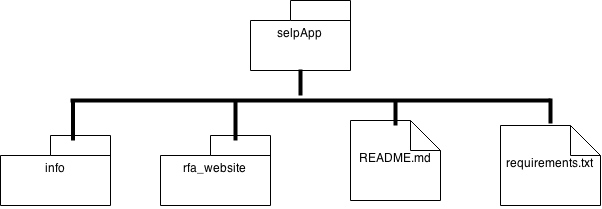
\includegraphics[scale=0.5]{selpProjectStructure.png} \\
\end{center}

Global deployment (especially via the described web hosting service \textit{Heroku} in a later section) would require more packages beyond those in the \verb|requirements.txt| to be installed as well as a few settings change to increase the security of the web application.

\subsubsection{The Django Project Directory}
The django project directory \verb|rfa_website| contains all of the code,the database (when created or the one submitted is used, both possibilities described in the quick start guide of the readme), and settings files necessary to get the web application running. The \verb|real_fantasy_adventure_app| directory holds all of the code for the Real Fantasy Adventure web application. I had purposefully split the files in their respective directories, and in the code (such as allowing the urls.py of the web application handle the url mapping within the application and only have the urls.py at website level shove the url mapping off to respective applications in order to decouple the code within the project as a whole as much as possible. Actually making it possible to install the real\_fantasy\_adventure\_app application portable between Django projects with minimal effort.


\section{Design Choices}
I have stuck to the design choices made in Part 1, with the exception of some of the packages that were installed in order to fulfill the requirements for a certain feature or make something easier. Most of these design choices were also made for the same reasons of inexperience in part 1. As I had expressed in the proposal I actually did spend 70\% of my time learning about web stacks, technologies, and idiomatic practices; and 30\% of my time on the implementation.

\subsection{Technologies}
\subsubsection{Python2.7.8}
I had decided on using Python2.7.8 because I felt most comfortable using this language in this version from past experience in it. Additionally this version worked well together with \textit{virtualenv} on DiCE machines, whereas there was a bug in the version of virtualenv installed on DiCE in the creation of the virtual environment if initialized with the installed Python3.4 version (at least by the time of this writing, I realize there is a pyenv workaround that has been described in the informatics website, but didnt find this until later) this I have stuck to my decision to use Python2.7.8 despite the suggestion to use the newer version in the proposal feedback. However my code has been kept general enough so that even a web server running the project in Python3.x should theoretically work without problem save for a few lines that may need to be updated. However I think it still is important to be critical of using an older language version when a newer one is present.

\subsubsection{Django 1.7}
I chose a heavier web development framework, Django1.7, because I saw it as an all-in-one package that contained a built-in web server, descriptive config that were easy to edit, a test suite that was easy to run, a large community of users, ORM functionality, and implementation language being python appealed to me greatly as a newcomer to web development. The availability and ease of installing plug ins to the framework was of great help to me in this practical. I spent a great amount of time making smaller applications (not this practical) in order to get used to the framework and initially found its strict Model-View-Template structure for data-driven applications a bit restrictive but over time have found its directed way of starting up applications helpful in getting applications on its feet quickly.

The ORM, and database migration management functionalities have made things much easier as curating a database manually would have taken me a lot of time to understand and perform. It is arguable that I may have learned even more about web technologies/development at a fundamental level had a taken a lighter framework such as \textit{flask} but I do not think I would have been able to create much of a project in the time I was given had I done so.

\subsubsection{HTML \& CSS with Django}
Having focused mainly on understanding the back-end handling of the web application with Django I ended up doing little in regards of making the web application pretty (though it would not be difficult to perform, for anyone who has a better design sense and html/css experience than I do). I have used html along with Django's templating system to create html pages with variable content pulled from the database to serve to the user instead of hard coded html. Additionally, using django's templating system I had all of the templates extend a base html file so that the general look of the website can be changed wholly simply by changing this base HTML file and the CSS files referenced by it. I have used a CSS bundle provided by the Skeleton CSS Boiler Plate (by Mr. Dave Gamache, under MIT License) project to style some aspects of the web application such as the buttons and forms, as I could not make it look good myself but was unwilling to use a larger package such as BootStrap without fully appreciating its strengths.
 
\subsubsection{SQLite3}
I have kept to using the standard database SQLite3 that is used by default for development in Django because I found it sufficient for my task and needs. Even in production I believe its use would be fine, as I don't expect many users of my application, and features involving concurrent updates and large scale calculations involving millions of rows is unlikely. Even so it would not be difficult to use another DBMS such as MySQL or PostGresQL as these are supported by Django and can be used after changing the rfa\_website/settings.py DATABASES variable, as well as changing some model fields as necessary.

\section{Development}
\subsection{Difficulties and Deficiencies}

\subsection{Things I am proud of}
\subsubsection{Usage of Git}
\subsubsection{Documentation}
DocStrings, lol sphinx improvement
\subsubsection{Tests}
Lots of unit tests, early start on model tests, say how late you were in view tests

\section{Implementation Choices}
\section{Current Functional Deficiencies}

\subsection{Suggested Improvements}

\subsubsection{Tests}


\section{Conclusion}

\section{\textit{Extra:} Deploying the Project Globally on Heroku}

\end{document}
